

\section{Hardware Device}
\begin{figure}[t]
\centering
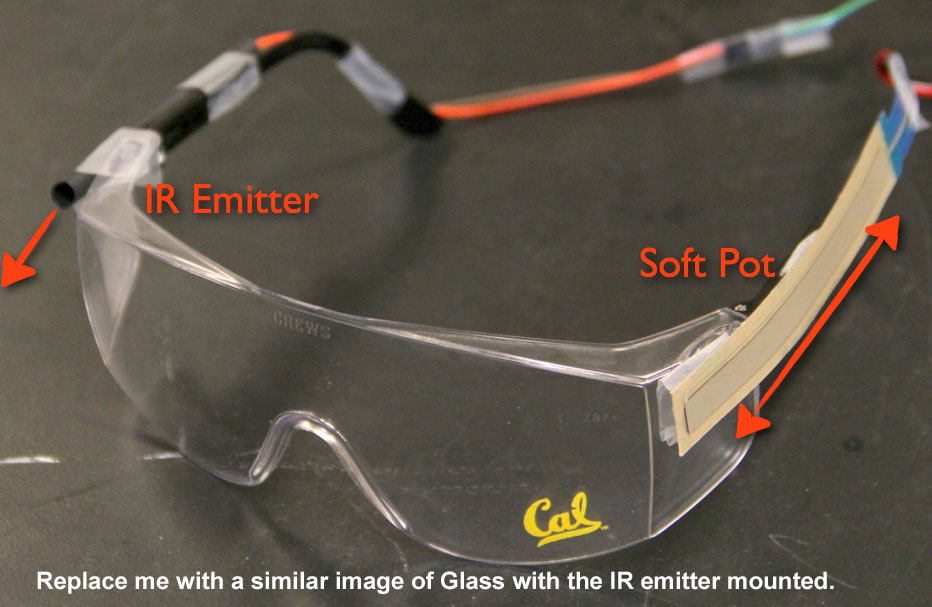
\includegraphics[width=1.0\columnwidth]{figures/glass-with-ir}
\caption{Our augmented Glass prototype has a frame-mounted infrared emitter.}
\label{fig:glass}
\end{figure}
\begin{figure}[t]
\centering
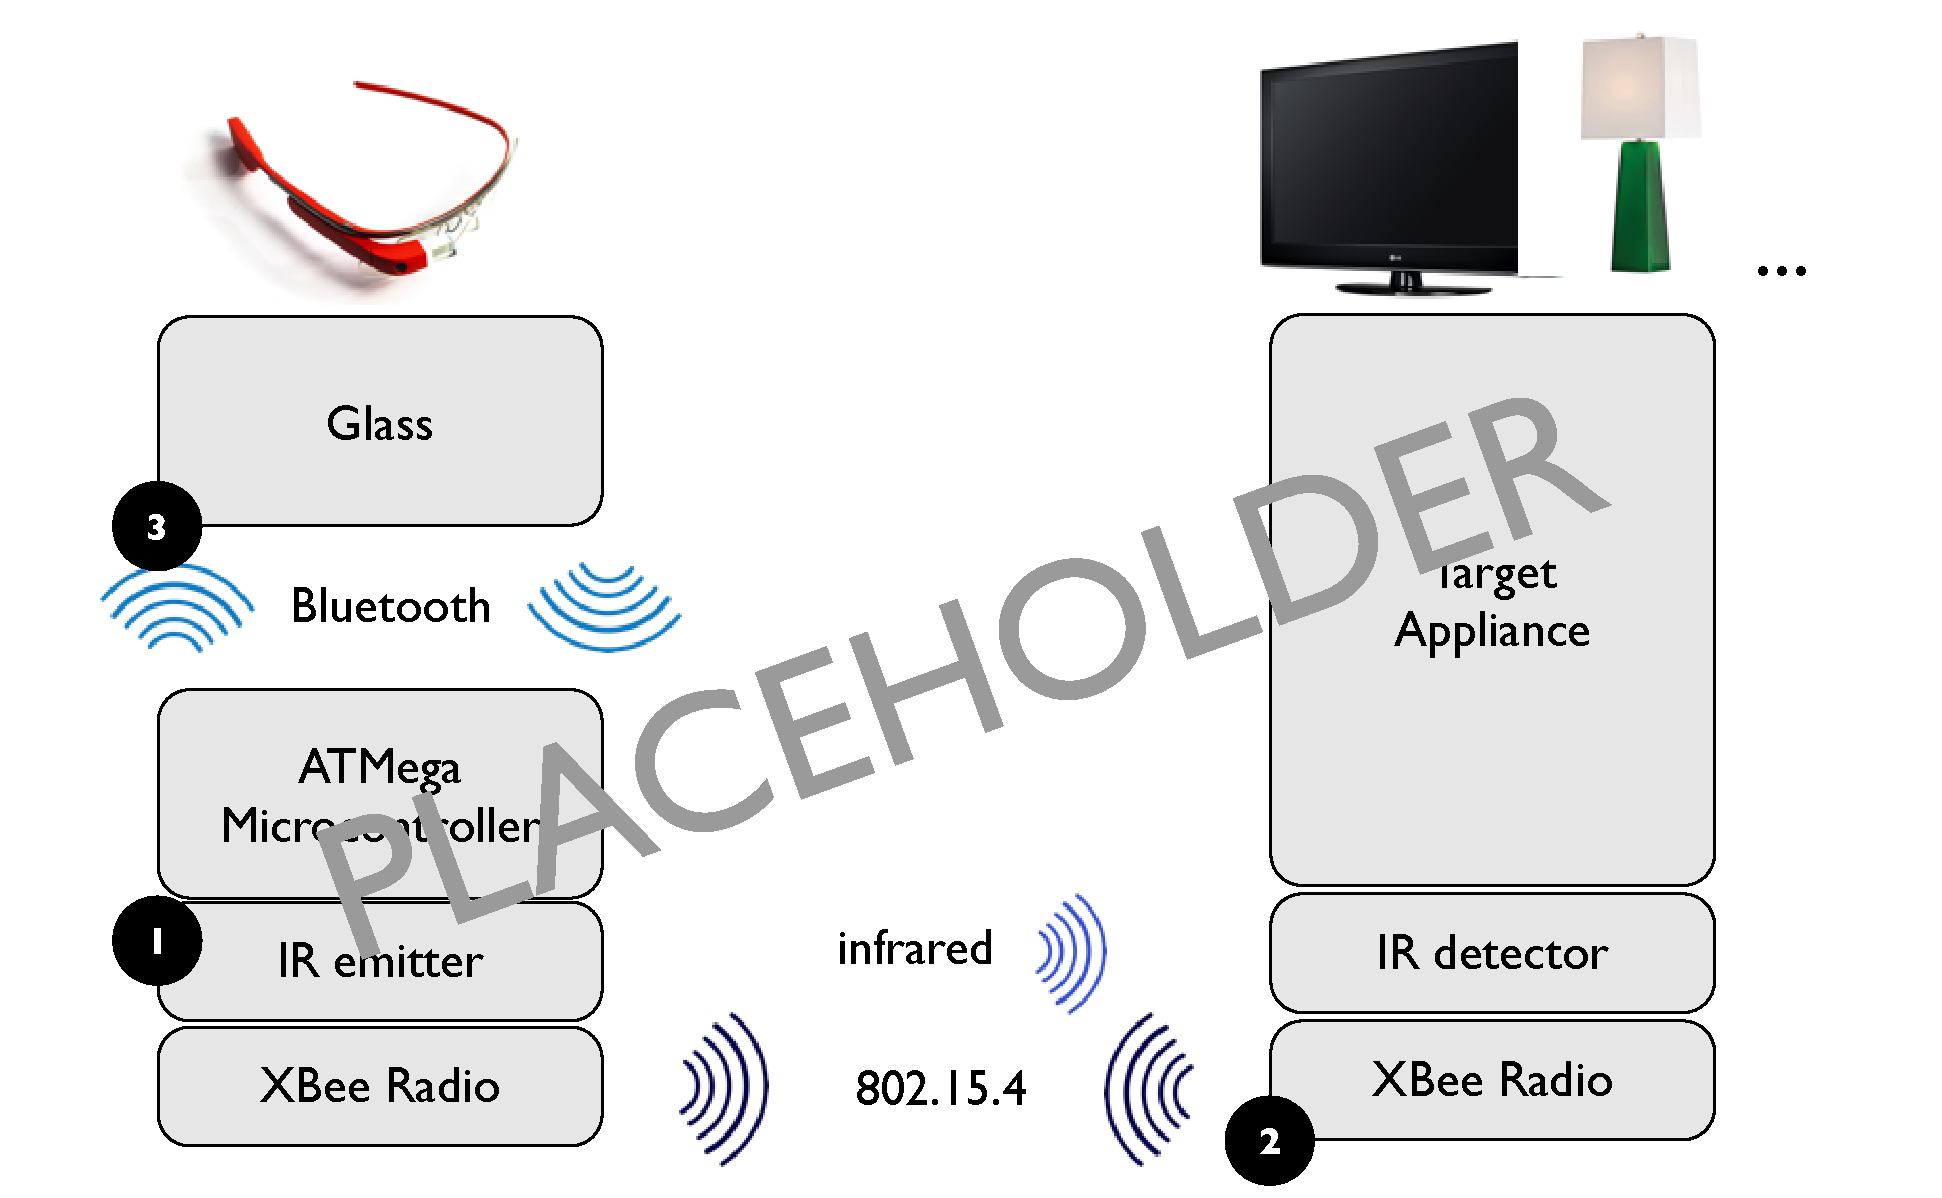
\includegraphics[width=1.0\columnwidth]{figures/architecture}
\caption{In our system architecture, selection is initiated through infrared but confirmed over 802.15.4. This permits wearers to move their head freely after connecting to an appliance. In the research prototype, users have to carry an additional microcontroller board that marshalls messages between Glass' Bluetooth radio an IR/802.15.4, but our custom hardware could also be integrated into the wearable device.}
\label{fig:architecture}
\end{figure}

\subsection{Prototype Implementation}
Our prototype consists of a Google Glass Explorer Edition head-worn computing device, augmented with an infrared emitter that is mounted on the frame, pointing out in the direction of the wearer's view (Figure~\ref{fig:glass}). The IR emitter LED is mounted in an opaque hollow tube, that restricts the outgoing angle of illumination. 

In our prototype, Glass communicates over Bluetooth to an additional microcontroller board the user has to wear (Atmel ATMega256). This board marshals XBee to Bluetooth messages in both directions and also controls the IR LED mounted on the Glass frame (Figure~\ref{fig:architecture}). This architecture was mostly chosen for reasons of expediency. We selected XBee 802.15.4 radios to avoid Bluetooth  wake up latencies but we do not claim optimality for our design decisions. Future head-mounted devices could clearly integrate IR emitters; the choice of local wireless technology could also change. In particular, one could substitute WiFi modules or design an all-Bluetooth network.

\subsection{Device Characterization}
We determined the usable range and accuracy empirically with one IR emitter and two IR receivers. The IR emitter constantly sent out an id signal. The receivers that correctly received the signal turn their LED on for 300 ms.

We placed all three devices at the same height with clear line of sight. The IR emitter is first places 2 feet away from the receivers. The receivers were moved sideways apart from each other until they could no longer receive stable signals. We then recorded the distance of the two receivers for the calculation of coverage angles. The steps are repeated for IR emitters in different distances (as shown in Table~\ref{table:measurements}). We then repeated measurements with the emitter  placed at various depths in the tube (see Figure~\ref{fig:coverage}). 

In summary, our measurements suggest that IR communication can be targeted to an area about 2--4' in diameter, up to 16' in front of the user. These values are a reasonable match for selecting appliances in a room-size environment. A wider beam would lead to an increased chance of multiple appliances receiving IR signals simultaneously. A narrower beam will make targeting more challenging, given the precision constraints of human head movement.

\afterpage{
\begin{figure}[t!]
\centering
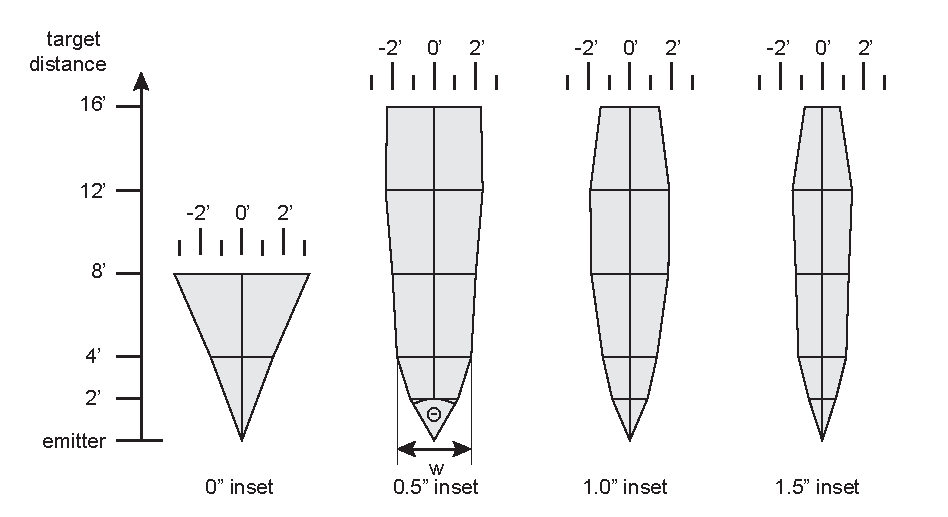
\includegraphics[width=1.0\columnwidth]{figures/glass-ir-coverage}
\caption{Different IR configurations suggest that usable beam widths of 2 to 4 feet and distances up to 16 feet }
\label{fig:coverage}
\end{figure}

\begin{table}[h!]
    \begin{tabular}{l|lllll}
    distance/ depth & \ft2       & \ft4       & \ft8   & \ft{12}  & \ft{16}  \\ \hline
    \inch{0}                     & $74\degree$ & $78\degree$ & N/A  & N/A  & N/A  \\
  \inch{0.5}                   & $60\degree$ & $48\degree$     & $28\degree$ & $22\degree$ & $16\degree$ \\
    \inch{1.0}                     & $46\degree$     & $36\degree$     & $26\degree$ & $18\degree$ & $10\degree$ \\
    \inch{1.5}                   & $36\degree$     & $32\degree$     & $18\degree$ & $14\degree$ & $6\degree$  \\
    \end{tabular}
    \caption{Measured IR coverage angles $\Theta$ at different target distances and different depths of IR emitter inside shielding tube.}
    \label{table:measurements}
\end{table}
} %end afterpage